\documentclass[nohyper]{tufte-handout}

%%encoding
%%---------------------------------------------------------
%\usepackage[utf8]{inputenc}
%\usepackage[T1]{fontenc}
%%----------------------------------------------------------------------

\usepackage{graphicx} % allow embedded images
  %\setkeys{Gin}{width=\linewidth,totalheight=\textheight,keepaspectratio}
  \graphicspath{{img/}} % set of paths to search for images
%\usepackage[english]{babel}
\usepackage{amsmath}
\usepackage{amsfonts}
\usepackage{amssymb}
%\usepackage{array}

\usepackage{booktabs} % book-quality tables
\usepackage{units}    % non-stacked fractions and better unit spacing
\usepackage{multicol} % multiple column layout facilities
\usepackage{fancyvrb} % extended verbatim environments
  \fvset{fontsize=\normalsize}% default font size for fancy-verbatim environments

\usepackage{url}
\usepackage{hyperref}
\hypersetup{colorlinks=true}
\usepackage{listings}
\usepackage{verbatim}
\usepackage[shortlabels]{enumitem}
%\usepackage{natbib}
%\setcitestyle{square, number}
\usepackage{xstring}
\usepackage{catchfile}
\usepackage{microtype}

\CatchFileDef{\headfull}{.git/HEAD}{}
\StrGobbleRight{\headfull}{1}[\head]
\StrBehind[2]{\head}{/}[\branch]
\CatchFileDef{\commit}{.git/refs/heads/\branch}{}


\begin{document}
\renewcommand{\abstractname}{\vspace{-\baselineskip}}

\title{Bitcoin: A Peer-to-Peer Electronic Cash System}
\author{Satoshi Nakamoto \footnotesize{({satoshin@gmx.com}, 
\href{http://www.bitcoin.org}{bitcoin.org})}}
\date{}


\maketitle

\marginnote[-1.2in]{GitHub: \href{https://github.com/chanhosuh/annotated-satoshi}{chanhosuh/annotated-satoshi}}
\marginnote[-1.05in]{commit \texttt{\StrLeft{\commit}{7}} on branch \texttt{\branch}.}

\begin{abstract}
\noindent
\marginnote[-0.6in]{The original whitepaper has no footnotes or margin notes.  We have added these to give further details or clarifications, including changes that have occurred in the Bitcoin implementation.\\ 
Suggestions and corrections to this document may be submitted via pull request at its GitHub repository.}
A purely peer-to-peer version of electronic cash would allow online payments to be sent directly from one party to another without going through a financial institution. Digital signatures provide part of the solution, but the main benefits are lost if a trusted third party is still required to prevent double-spending.We propose a solution to the double-spending problem using a peer-to-peer network. The network timestamps transactions by hashing them into an ongoing chain of hash-based proof-of-work, forming a record that cannot be changed without redoing the proof-of-work. The longest chain not only serves as proof of the sequence of events witnessed, but proof that it came from the largest pool of CPU power\footnote{Due to the prevalence of specialized equipment such as ASIC miners, references to "CPU power" should be replaced by "hashrate", i.e. the number of \texttt{sha256} operations per unit time.}. As long as a majority of CPU power is controlled by nodes that are not cooperating to attack the network, they'll generate the longest chain and outpace attackers. The network itself requires minimal structure. Messages are broadcast on a best effort basis, and nodes can leave and rejoin the network at will, accepting the longest proof-of-work chain as proof of what happened while they were gone. 
\end{abstract}


\section{Introduction}\label{introduction}

\newthought{Commerce on the Internet} has come to rely almost exclusively on
financial institutions serving as trusted third parties to process
electronic payments. While the system works well enough for most
transactions, it still suffers from the inherent weaknesses of the trust
based model. Completely non-reversible transactions are not really
possible, since financial institutions cannot avoid mediating disputes.
The cost of mediation increases transaction costs, limiting the minimum
practical transaction size and cutting off the possibility for small
casual transactions, and there is a broader cost in the loss of ability
to make non-reversible payments for nonreversible services. With the
possibility of reversal, the need for trust spreads. Merchants must be
wary of their customers, hassling them for more information than they
would otherwise need. A certain percentage of fraud is accepted as
unavoidable. These costs and payment uncertainties can be avoided in
person by using physical currency, but no mechanism exists to make
payments over a communications channel without a trusted party

What is needed is an electronic payment system based on cryptographic
proof instead of trust, allowing any two willing parties to transact
directly with each other without the need for a trusted third party.
Transactions that are computationally impractical to reverse would
protect sellers from fraud, and routine escrow mechanisms could easily
be implemented to protect buyers. In this paper, we propose a solution
to the double-spending problem using a peer-to-peer distributed
timestamp server to generate computational proof of the chronological
order of transactions.  \footnote{Satoshi emphasizes his solution is a timestamp server which orders data.  Proof-of-work (POW) provides a consensus mechanism for securing the ordered data. This shows Satoshi understands that digital currency is just one application of blockchain technology.} The system is secure as long as honest nodes
collectively control more CPU power than any cooperating group of
attacker nodes.

\section{Transactions}\label{transactions}

\newthought{We define} an electronic coin as a chain of digital signatures.
\footnote{
Every bitcoin address is actually the hash of a locking script, or \emph{encumbrance}, which can be opened with the appropriate unlocking script.   Locking and unlocking scripts, are written in a language Satoshi called simply "Script".\\
Whenever the text reads "signature", you should think of "unlocking script"; similarly, wherever "public key" arises, think of "locking script".  In Bitcoin parlance, the unlocking script is called \texttt{scriptSig} and the locking script is called \texttt{scriptPubKey}, in recognition of the most common case where the signature is needed to unlock spending to a public key.\\
Script allows more complex transfers than a sender to a single recipient.  More general encumbrances could be multi-signature or require the solution to a puzzle, such as pre-image to a hash function.
}

Each owner transfers the coin to the next by digitally signing a hash of the
previous transaction and the public key of the next owner and adding
these to the end of the coin. A payee can verify the signatures to
verify the chain of ownership.

\begin{figure}[!h]
\centering
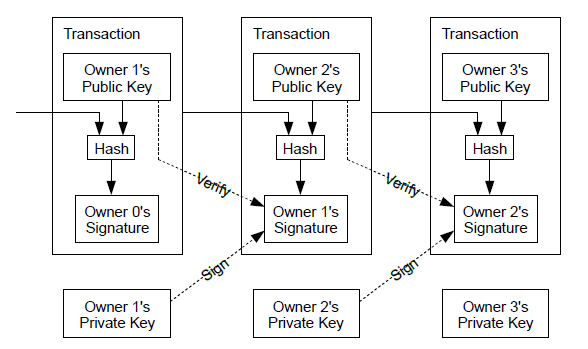
\includegraphics[width=0.75\linewidth]{transactions.png}
\end{figure}

The problem of course is the payee can't verify that one of the owners did not double-spend the coin. A common solution is to introduce a trusted central authority, or mint, that checks every transaction for double spending. After each transaction, the coin must be returned to the mint to issue a new coin, and only coins issued directly from the mint are trusted not to be double-spent. The problem with this solution is that the fate of the entire money system depends on the company running the mint, with every transaction having to go through them, just like a bank.

We need a way for the payee to know that the previous owners did not
sign any earlier transactions. For our purposes, the earliest
transaction is the one that counts, so we don't care about later
attempts to double-spend. The only way to confirm the absence of a
transaction is to be aware of all transactions. In the mint based model, the mint was aware of all transactions and decided which arrived first.
To accomplish this without a trusted party, transactions must be
publicly announced\cite[-0.1in]{dai98}, and we need a system for participants to agree on a single history of the order in which they were received. The payee needs proof that at the time of each transaction, the majority of nodes agreed it was the first received.

\section{Timestamp Server}\label{timestamp-server}

\newthought{The solution} we propose begins with a timestamp server. A timestamp
server works by taking a hash of a block of items to be timestamped and
widely publishing the hash, such as in a newspaper or Usenet
post\cite[-1.5in]{mas99}\cite[-0.625in]{hab90}\cite[-0.2in]{bay93}\cite[0in]{hab97}. The timestamp proves that the data must have existed
at the time, obviously, in order to get into the hash. Each timestamp
includes the previous timestamp in its hash, forming a chain, with each
additional timestamp reinforcing the ones before it.

\begin{figure}[!h]
\centering
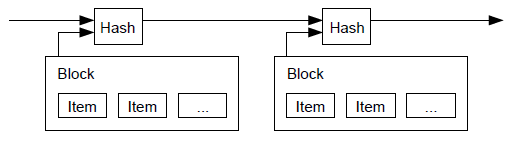
\includegraphics[width=0.75\linewidth]{timestamp.png}
\end{figure}

\section{Proof-of-Work}\label{proof-of-work}

\newthought{To implement} a distributed timestamp server on a peer-to-peer basis, we
will need to use a proof-of-work system similar to Adam Back's Hashcash
\cite[-0.75in]{bac02}, rather than newspaper or Usenet posts. The
proof-of-work involves scanning for a value that when hashed, such as
with SHA-256, the hash begins with a number of zero bits. The average
work required is exponential in the number of zero bits required and can be verified by executing a single hash.



For our timestamp network, we implement the proof-of-work by
incrementing a nonce\footnote[][-1.3in]{At current difficulty levels, the nonce's 4 bytes do not provide enough hashes, so miners must vary the input data another way, e.g., re-ordering transactions or changing the timestamp.\\In practice, miners use the \emph{extranonce}, a portion of the coinbase input's \texttt{scriptSig}.  This \texttt{scriptSig} not only houses the extranonce, but starts with the block height, due to BIP 34, to disallow a transaction duplication. } in the block until a value is found that gives the
block's hash\footnote[][0.1in]{It is the block header, not the block itself, that is hashed.  A block is comprised of the header followed by the list of transactions.}
the required zero bits. Once the CPU effort has been
expended to make it satisfy the proof-of-work, the block cannot be
changed without redoing the work. As later blocks are chained after it,
the work to change the block would include redoing all the blocks after
it.

\marginnote[0.1in]{
\noindent\fbox{%
    \parbox{2.45in}{%
Block header:\\[0.04in]

\textcolor{blue}{00c0ff3f}\textcolor{red}{6452255a2f9c192c4f0cb09029058bf427c295d0\\4bc109000000000000000000}\textcolor{cyan}{581267a8e88b6c7c8234af\\c16cc089e2ebbacc177ec018ff4498398e1115b3c5}\textcolor{magenta}{f9da3\\45e}\textcolor{teal}{ff321217}\textcolor{lime}{3b247c3d}
}
}

version - \textcolor{blue}{00c0ff3f}\\
prev block header hash - \textcolor{red}{6452255...}\\
merkle root - \textcolor{cyan}{581267a...}\\
time - \textcolor{magenta}{f9da345e}\\
nBits - \textcolor{teal}{ff321217}\\
nonce - \textcolor{lime}{3b247c3d}\\

Block header hash:\\
\textcolor{darkgray}{00000000000000000002f01e49c839b\\
7e13be20fba241f112e9a4634c4ece2c0}
}


\begin{figure}[!h]
\centering
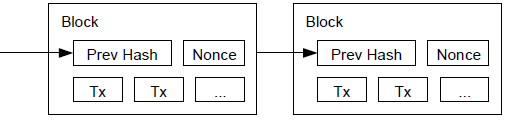
\includegraphics[width=0.75\linewidth]{proof-of-work.png}
\end{figure}

The proof-of-work also solves the problem of determining representation
in majority decision making. If the majority were based on
one-IP-address-one-vote, it could be subverted by anyone able to
allocate many IPs. Proof-of-work is essentially one-CPU-one-vote. The
majority decision is represented by the longest chain, which has the greatest proof-of-work effort invested in it.\footnote{By "longest chain" Satoshi always means the chain with the greatest total POW.  This is essentially the sum of the difficulties of the blocks.  More precisely, it is the expected value of the number of hashes needed to produce a chain of blocks of those particular difficulties.} If a majority of CPU power is controlled by honest nodes, the honest chain will grow the fastest and outpace any competing chains. To modify a past block, an attacker would have to redo the proof-of-work of the block and all blocks after
it and then catch up with and surpass the work of the honest nodes. We will show later that the probability of a slower attacker catching up
diminishes exponentially as subsequent blocks are added.


To compensate for increasing hardware speed and varying interest in running nodes over time, the proof-of-work difficulty\footnote{Difficulty is defined as a constant multiplied by the reciprocal of the \emph{target}, which is a 32 byte integer.  A block is successful mined when the block header hash is below the target value.
} is determined by a moving average targeting an average number of blocks per hour.\footnote{The difficulty adjustment is not based on a moving average but on comparing the elapsed time to mine 2,016 blocks with the expected time.  Every 2,016 block mined has a new difficulty calculated by multiplying the old difficulty by the ratio of expected time to actual time.  More precisely: $$ \text{new difficulty} = \text{old difficulty} \cdot \left( \frac{\text{expected time}}{\text{actual time}}\right)$$ Also, to keep difficulty from varying abruptly, the adjustment is limited by a factor of 4: $$1/4 <= \frac{\text{new difficulty}}{\text{old difficulty}} <= 4$$

"Actual time" is defined as the difference in the timestamps of the last and first of the 2016 blocks.  This is not expected to be a very accurate measure of time, as the rules for timestamping are generous, but suffices for difficulty adjustment.
 }   If they're generated too fast, the difficulty increases.

\section{Network}\label{network}

The steps to run the network are as follows:

\begin{enumerate}[1)]
\item
  New transactions are broadcast to all nodes.
\item
  Each node collects new transactions into a block.
\item
  Each node works on finding a difficult proof-of-work for its block.
\item
  When a node finds a proof-of-work, it broadcasts the block to all
  nodes.
\item
  Nodes accept the block only if all transactions in it are valid and
  not already spent.
\item
  Nodes express their acceptance of the block by working on creating the
  next block in the chain, using the hash of the accepted block as the
  previous hash.
\end{enumerate}

Nodes always consider the longest chain to be the correct one and will keep working on extending it. If two nodes broadcast different versions of the next block simultaneously, some nodes may receive one or the other first. In that case, they work on the first one they received, but save the other branch in case it becomes longer. The tie will be broken when the next proof-of-work is found and one branch becomes longer; the
nodes that were working on the other branch will then switch to the longer one.

New transaction broadcasts do not necessarily need to reach all nodes.
As long as they reach many nodes, they will get into a block before long. Block broadcasts are also tolerant of dropped messages. If a node does not receive a block, it will request it when it receives the next block and realizes it missed one.

\section{Incentive}\label{incentive}

\newthought{By convention}, the first transaction in a block is a special transaction
that starts a new coin owned by the creator of the block.  \footnote{This is the \emph{coinbase} transaction.  It has exactly one input which refers to a null outpoint.  The \texttt{scriptSig} for the input, confusingly referred to as the "coinbase", allows up to 100 bytes of data.\\By BIP 34, this data must include the block height.  The "extra nonce" is also part of the data, as the nonce field in the block header is not sufficient for mining at current difficulties.\\Besides the output to pay the miner, Segwit mandates an additional output with \texttt{OP\_RETURN} script containing a commitment to the witness data. } This adds an
incentive for nodes to support the network, and provides a way to
initially distribute coins into circulation, since there is no central
authority to issue them. The steady addition of a constant of amount of
new coins is analogous to gold miners expending resources to add gold to
circulation. In our case, it is CPU time and electricity that is
expended.

The incentive can also be funded with transaction fees. If the output
value of a transaction is less than its input value, the difference is a
transaction fee that is added to the incentive value of the block
containing the transaction. Once a predetermined number of coins have
entered circulation, the incentive can transition entirely to
transaction fees and be completely inflation free.

The incentive may help encourage nodes to stay honest. If a greedy
attacker is able to assemble more CPU power than all the honest nodes,
he would have to choose between using it to defraud people by stealing
back his payments, or using it to generate new coins. He ought to find
it more profitable to play by the rules, such rules that favour him with
more new coins than everyone else combined, than to undermine the system
and the validity of his own wealth.  \footnote[][-1in]{This still leaves the system vulnerable to a "Goldfinger attack", e.g. any attack motivated by political or ideological motives.}

\section{Reclaiming Disk Space}\label{reclaiming-disk-space}

\newthought{Once the latest} transaction in a coin is buried under enough blocks, the
spent transactions before it can be discarded to save disk space. To
facilitate this without breaking the block's hash, transactions are
hashed in a Merkle Tree\cite[-1.7in]{mer80}\cite[-1.1in]{mas99}\cite[-0.25in]{hab97}, with only the root included in the block's hash. Old
blocks can then be compacted by stubbing off branches of the tree. The
interior hashes do not need to be stored.

\begin{figure}[!h]
\centering
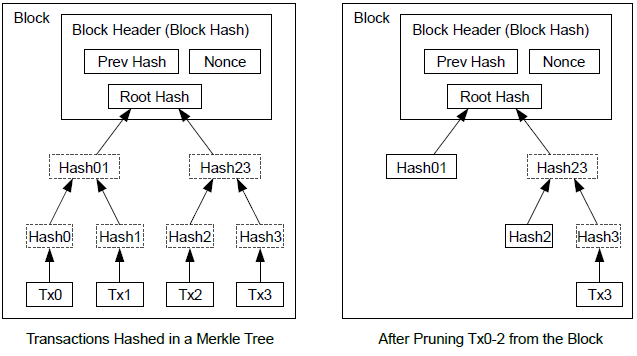
\includegraphics[width=0.75\linewidth]{reclaiming-disk.png}
\end{figure}

A block header with no transactions would be about 80 bytes.  \footnote{A block header is in fact precisely 80 bytes.} If we
suppose blocks are generated every 10 minutes\footnote{The difficulty adjustment is based on an average value of 10 minutes to mine a block.}, 80 bytes * 6 * 24 * 365 =
4.2MB per year. With computer systems typically selling with 2GB of RAM
as of 2008, and Moore's Law predicting current growth of 1.2GB per year,
storage should not be a problem even if the block headers must be kept
in memory.


\section{Simplified Payment
Verification}\label{simplified-payment-verification}

\newthought{It is possible} to verify payments without running a full network node.\footnote{By "full network node", Satoshi means node that does full validation alongside mining.  The original Bitcoin client required mining.  Current version of Bitcoin Core allow a node to run full validation on blocks without mining.} A user only needs to keep a copy of the block headers of the longest
proof-of-work chain, which he can get by querying network nodes until
he's convinced he has the longest chain, and obtain the Merkle branch
linking the transaction to the block it's timestamped in. He can't check
the transaction for himself, but by linking it to a place in the chain,
he can see that a network node has accepted it, and blocks added after
it further confirm the network has accepted it.

\begin{figure}[!h]
\centering
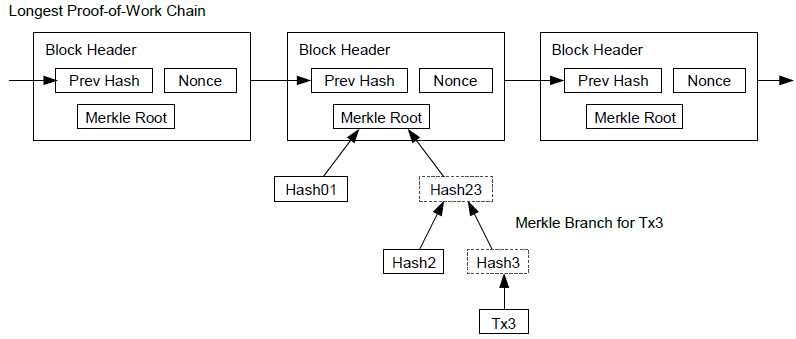
\includegraphics[width=\linewidth]{spv.png}

\end{figure}

As such, the verification is reliable as long as honest nodes control
the network, but is more vulnerable if the network is overpowered by an
attacker.  \footnote[][-0.5in]{With the current p2p protocol, a light node needs to connect to only one honest node to recognize the main chain.  So a "Sybil attack" can only be successful if the light node is completely isolated from honest nodes.} While network nodes can verify transactions for themselves,
the simplified method can be fooled by an attacker's fabricated
transactions for as long as the attacker can continue to overpower the
network. One strategy to protect against this would be to accept alerts
from network nodes when they detect an invalid block, prompting the
user's software to download the full block and alerted transactions to
confirm the inconsistency. Businesses that receive frequent payments
will probably still want to run their own nodes for more independent
security and quicker verification.

\section{Combining and Splitting
Value}\label{combining-and-splitting-value}

\newthought{Although} it would be possible to handle coins individually, it would be
unwieldy to make a separate transaction for every cent in a transfer. To
allow value to be split and combined, transactions contain multiple
inputs and outputs. Normally there will be either a single input from a
larger previous transaction or multiple inputs combining smaller
amounts, and at most two outputs: one for the payment, and one returning
the change, if any, back to the sender.

\begin{figure}[!h]
\centering
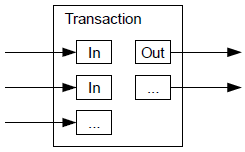
\includegraphics[width=0.3725\linewidth]{combining-splitting.png}

\end{figure}

It should be noted that fan-out, where a transaction depends on several
transactions, and those transactions depend on many more, is not a
problem here. There is never the need to extract a complete standalone
copy of a transaction's history.

\section{Privacy}\label{privacy}

\newthought{The traditional banking} model achieves a level of privacy by limiting access to information to the parties involved and the trusted third party. The necessity to announce all transactions publicly precludes this method, but privacy can still be maintained by breaking the flow of information in another place: by keeping public keys anonymous. The public can see that someone is sending an amount to someone else, but without information linking the transaction to anyone. This is similar to the level of information released by stock exchanges, where the time and size of individual trades, the ``tape'', is made public, but without telling who the parties were.

\begin{figure}[!h]
\centering
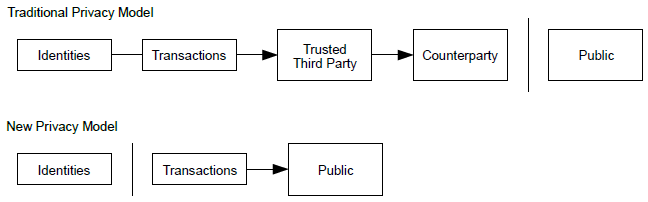
\includegraphics[width=0.75\linewidth]{privacy.png}
\end{figure}

As an additional firewall, a new key pair should be used for each
transaction to keep them from being linked to a common owner.  \footnote{Hierarchical deterministic (HD) wallets provide this protection by generating an essentially infinite supply of keys for use from a root seed, usually represented by a 24 word mnemonic (BIP ?).} Some
linking is still unavoidable with multi-input transactions, which
necessarily reveal that their inputs were owned by the same owner. The
risk is that if the owner of a key is revealed, linking could reveal
other transactions that belonged to the same owner.  \footnote{Satoshi recognizes the danger of "linking", but he does not propose a solution.}

\section{Calculations}\label{calculations}

\newthought{We consider} the scenario of an attacker trying to generate an alternate
chain faster than the honest chain. Even if this is accomplished, it
does not throw the system open to arbitrary changes, such as creating
value out of thin air or taking money that never belonged to the
attacker. Nodes are not going to accept an invalid transaction as
payment, and honest nodes will never accept a block containing them. An
attacker can only try to change one of his own transactions to take back
money he recently spent.

The race between the honest chain and an attacker chain can be
characterized as a Binomial Random Walk. The success event is the honest
chain being extended by one block, increasing its lead by +1, and the
failure event is the attacker's chain being extended by one block,
reducing the gap by -1.

The probability of an attacker catching up from a given deficit is
analogous to a Gambler's Ruin problem. Suppose a gambler with unlimited
credit starts at a deficit and plays potentially an infinite number of
trials to try to reach breakeven. We can calculate the probability he
ever reaches breakeven, or that an attacker ever catches up with the
honest chain, as follows\cite{fel57}:

\

\(p\) = {\small probability an honest node finds the next block}

\(q\) = {\small probability the attacker finds the next block}

\(q_z\) = {\small probability the attacker will ever catch up from z blocks behind}

\begin{equation}
    q_z = 
\begin{cases}
    1               & \text{if } p \leqslant q\\
    \left(q/p\right)^z & \text{if } p > q
\end{cases}
\end{equation}

\

Given our assumption that $p > q$, the probability drops
exponentially as the number of blocks the attacker has to catch up with
increases. With the odds against him, if he doesn't make a lucky lunge
forward early on, his chances become vanishingly small as he falls
further behind.

We now consider how long the recipient of a new transaction needs to
wait before being sufficiently certain the sender can't change the
transaction. We assume the sender is an attacker who wants to make the
recipient believe he paid him for a while, then switch it to pay back to
himself after some time has passed. The receiver will be alerted when
that happens, but the sender hopes it will be too late

The receiver generates a new key pair and gives the public key to the
sender shortly before signing. This prevents the sender from preparing a
chain of blocks ahead of time by working on it continuously until he is
lucky enough to get far enough ahead, then executing the transaction at
that moment. Once the transaction is sent, the dishonest sender starts
working in secret on a parallel chain containing an alternate version of
his transaction.

The recipient waits until the transaction has been added to a block and
$z$ blocks have been linked after it. He doesn't know the exact amount of
progress the attacker has made, but assuming the honest blocks took the
average expected time per block, the attacker's potential progress will
be a Poisson distribution with expected value:\footnote{The assumption on the time to generate the honest blocks nails down the number of hashes the honest miners needed.  Since the attacker's hashrate is in ratio $\frac{q}{p}$, this gives the formula for $\lambda$.  Technically it may be more correct to consider a binomial distribution here, but the Poisson distribution is a very good approximation and is more handy for calculations here.}

\begin{equation}
\lambda = z \ \frac{q}{p}
\end{equation}

\

To get the probability the attacker could still catch up now, we
multiply the Poisson density for each amount of progress he could have
made by the probability he could catch up from that point:

\begin{equation}
\sum _{k=0}^\infty \frac{\lambda ^k e^{-\lambda}}{k!} \cdot 
\begin{cases}
    \left(q/p\right)^{(z-p)} & \text{if } k \leqslant z \\
    1                     & \text{if } k > z
\end{cases}
\end{equation}

\

Rearranging to avoid summing the infinite tail of the
distribution\ldots{}

 
\begin{equation}
1 - \sum _{k=0}^z \frac{\lambda ^k e^{-\lambda}}{k!} \left(1 - \left(q/p\right)^{(z-k)}\right)
\end{equation}

\

Converting to C code\ldots{}

\

\lstset{ 
    language=C, % choose the language of the code
     basicstyle=\ttfamily,
       columns=fullflexible,
    numbers=none, % where to put the line-numbers
    numberstyle=\tiny, % the size of the fonts that are used for the line-numbers     
    showspaces=false, % show spaces adding particular underscores
    showstringspaces=false, % underline spaces within strings
    showtabs=false, % show tabs within strings adding particular underscores
    frame=single, % adds a frame around the code
    tabsize=4, % sets default tabsize to 2 spaces
    captionpos=b, % sets the caption-position to bottom
    breaklines=true, % sets automatic line breaking
    breakatwhitespace=false, 
    backgroundcolor=\color{gray!8},  
}

\begin{lstlisting}
#include <math.h>
double AttackerSuccessProbability(double q, int z)
{
    double p = 1.0 - q;
    double lambda = z * (q / p);
    double sum = 1.0;
    int i, k;
    for (k = 0; k <= z; k++)
    {
        double poisson = exp(-lambda);
        for (i = 1; i <= k; i++)
            poisson *= lambda / i;
        sum -= poisson * (1 - pow(q / p, z - k));
    }
    return sum;
}
\end{lstlisting}

\

Running some results, we can see the probability drop off exponentially
with $z$.

\

\begin{verbatim}
q=0.1
z=0 P=1.0000000
z=1 P=0.2045873
z=2 P=0.0509779
z=3 P=0.0131722
z=4 P=0.0034552
z=5 P=0.0009137
z=6 P=0.0002428
z=7 P=0.0000647
z=8 P=0.0000173
z=9 P=0.0000046
z=10 P=0.0000012


q=0.3
z=0 P=1.0000000
z=5 P=0.1773523
z=10 P=0.0416605
z=15 P=0.0101008
z=20 P=0.0024804
z=25 P=0.0006132
z=30 P=0.0001522
z=35 P=0.0000379
z=40 P=0.0000095
z=45 P=0.0000024
z=50 P=0.0000006
\end{verbatim}

\

Solving for $P$ less than 0.1\%\ldots{}\marginnote{This table is apparently the basis for the "6 confirmations" rule-of-thumb.  Note, however, that it only shows that 6 confirmations gives less than a 0.1\% chance of fraud for an attacker with 10\% of the hashrate.  Fending off a stronger attacker, such as one of the major mining pools, or reducing the chance of fraud to less than 1 in a 1000 would require significantly more confirmations.}

\

\begin{verbatim}
P < 0.001
q=0.10 z=5
q=0.15 z=8
q=0.20 z=11
q=0.25 z=15
q=0.30 z=24
q=0.35 z=41
q=0.40 z=89
q=0.45 z=340
\end{verbatim}


\section{Conclusion}\label{conclusion}

\newthought{We have proposed} a system for electronic transactions without relying on
trust. We started with the usual framework of coins made from digital
signatures, which provides strong control of ownership, but is
incomplete without a way to prevent double-spending. To solve this, we
proposed a peer-to-peer network using proof-of-work to record a public
history of transactions that quickly becomes computationally impractical
for an attacker to change if honest nodes control a majority of CPU
power. The network is robust in its unstructured simplicity. Nodes work
all at once with little coordination. They do not need to be identified,
since messages are not routed to any particular place and only need to
be delivered on a best effort basis. Nodes can leave and rejoin the
network at will, accepting the proof-of-work chain as proof of what
happened while they were gone. They vote with their CPU power,
expressing their acceptance of valid blocks by working on extending them
and rejecting invalid blocks by refusing to work on them. Any needed
rules and incentives can be enforced with this consensus mechanism.

\bibliography{refs}
\bibliographystyle{plainnat}

\end{document}
